\chapter{METODOLOGIA}

A metodologia utilizada no projeto é a exploratória.

Segundo \citeonline{VENTURA2007}, são verificadas grandes utilidades em estudos de casos realizados através de pesquisas exploratórias.

\begin{quoting}[rightmargin=0cm,leftmargin=4cm]
\begin{singlespace}
{\footnotesize  
“Por sua flexibilidade, é recomendável nas fases iniciais de uma investigação sobre temas complexos, para a construção de hipóteses ou reformulação do problema. Também se aplica com pertinência nas situações em que o objeto de estudo já é suficientemente conhecido a ponto de ser enquadrado em determinado tipo ideal. São úteis também na exploração de novos processos ou comportamentos, novas descobertas, porque têm a importante função de gerar hipóteses e construir teorias. Ou ainda, pelo fato de explorar casos atípicos ou extremos para melhor compreender os processos típicos \cite{VENTURA2007}.”
}
\end{singlespace}
\end{quoting}

\begin{comment}
Este estudo tem por finalidade apresentar resultados qualitativos sobre o assunto de visão computacional, visando explorar a didática e o conteúdo metodológico relacionado similarmente à pesquisa.

A pesquisa qualitativa será realizada baseada no livro \textit{Digital Image Processing} \cite{GONZALEZ2002}. Este livro fora escolhido para transmitir o conceito científico e teórico sobre o assunto de visão computacional. O segundo livro que será utilizado para extrair maiores informações sobre o assunto é o Processamento Digital de Imagens \cite{FILHO1999}, que também aborda conteúdos didáticos e científicos sobre o assunto, explicando a funcionalidade da visão computacional, como esta trabalha e a resolução dos problemas sucintos.

Outro livro que será utilizado para a síntese de informações é o \textit{Computer Vision: Algorithms and Applications} \cite{SZELISKI2010}, que cita relações sobre o assunto de forma clara e objetiva.

Portanto, a pesquisa relacionada ao tema desse trabalho será baseada em todos os livros descritos e alguns artigos, com a finalidade de desenvolver o conteúdo teórico sobre o assunto de forma à fácil entendimento.

\end{comment}

Sendo assim, será feito um estudo bibliográfico a partir do tema de visão computacional utilizando o acervo disponível sobre o assunto, com a finalidade de reunir informações para obter melhores resultados.

A pesquisa qualitativa será baseada principalmente nos três livros escolhidos: \textit{Digital Image Processing} \cite{GONZALEZ2002},  \textit{Computer Vision: Algorithms and Applications} \cite{SZELISKI2010} e Processamento Digital de Imagens \cite{FILHO1999}. Todos os livros foram escolhidos por transmitirem conceitos científicos, didáticos, teóricos e práticos sobre o assunto de visão computacional.

O desenvolvimento da aplicação proposta será feito através do estudo realizado sobre o tema. A aplicação será desenvolvida utilizando metodologia de desenvolvimento ágil, ou seja, será feita o planejamento de cada etapa de funcionamento do sistema, na qual o objetivo de cada entrega é proporcionar uma prévia do funcionamento do \textit{software}. Essa ação foi tomada para que a evolução do sistema seja gradativa e eficiente.

Para resumir a elaboração deste projeto, foi feito uma imagem ilustrativa da metodologia utilizada no decorrer das etapas de desenvolvimento deste:

\clearpage
\begin{figure}[!htb]
\caption{ {\footnotesize Metodologia de desenvolvimento do projeto.}}
 
\centering % para centralizarmos a figura
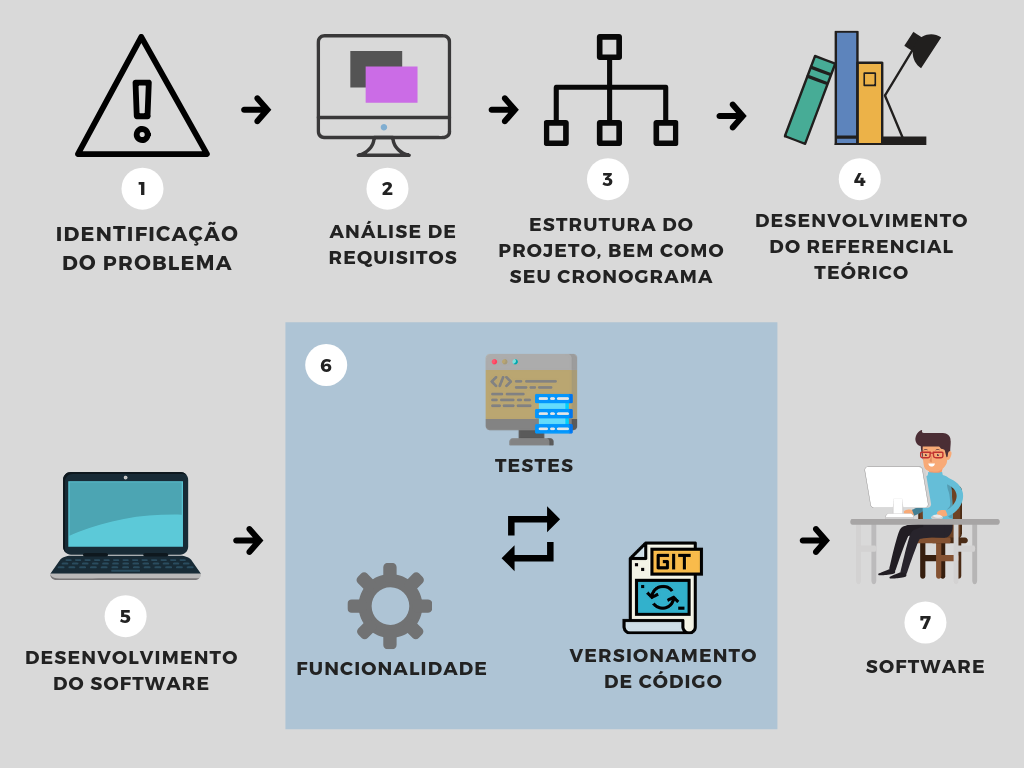
\includegraphics[width=15cm]{revisao-bibliografica/Figuras/Metodologia_TCC.png}% leia abaixo
\label{figura:figuraMet}

\centering \subfloat {\footnotesize { Fonte: Feita pelos autores do projeto. }}
{
\label{figura:figura7}
}
\end{figure}